\documentclass[tikz,border=6pt]{standalone}

\usepackage{amsmath}
\usepackage{tikz}
\usetikzlibrary{arrows.meta, positioning, calc, decorations.pathreplacing}

\begin{document}
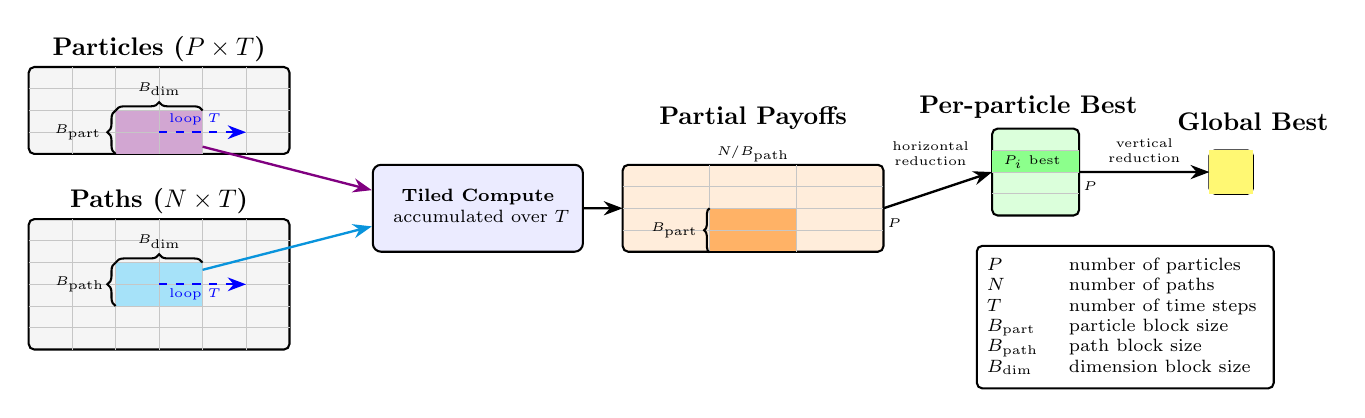
\begin{tikzpicture}[
    font=\scriptsize,
    >=Stealth,
    line width=0.75pt,
    scale=0.92,
    transform shape,
    box/.style={
        draw,
        rounded corners=2pt,
        fill=gray!8
    },
    compute/.style={
        draw,
        rounded corners=3pt,
        fill=blue!8,
        minimum width=2.9cm,
        minimum height=1.2cm,
        align=center
    },
    partial/.style={
        draw,
        rounded corners=2pt,
        fill=orange!14
    },
    reducebox/.style={
        draw,
        rounded corners=2pt,
        fill=green!14
    },
    outbox/.style={
        draw,
        rounded corners=2pt,
        fill=yellow!18
    },
    legendbox/.style={
        draw,
        rounded corners=2pt,
        fill=white,
        align=left
    },
    arr/.style={->, line width=0.85pt},
    gridline/.style={draw=gray!45, line width=0.3pt}
]

% Particles Grid: 4 x 6
\node[font=\bfseries] at (1.8,5.25) {Particles ($P \times T$)};
\coordinate (Psw) at (0,3.8);
\coordinate (Pne) at (3.6,5.0);
\draw[box] (Psw) rectangle (Pne);

\fill[violet!35] ($(Psw)+(1.2,0.0)$) rectangle ($(Psw)+(2.4,0.6)$);

\foreach \x in {0.6,1.2,1.8,2.4,3.0}
    \draw[gridline] ($(Psw)+(\x,0)$) -- ($(Psw)+(\x,1.2)$);
\foreach \y in {0.3,0.6,0.9}
    \draw[gridline] ($(Psw)+(0,\y)$) -- ($(Psw)+(3.6,\y)$);

\draw[decorate,decoration={brace,amplitude=3pt}]
    ($(Psw)+(1.2,0.0)$) -- ($(Psw)+(1.2,0.6)$)
    node[midway,left,xshift=-2pt,font=\tiny] {$B_{\text{part}}$};

\draw[decorate,decoration={brace,amplitude=3pt}]
    ($(Psw)+(1.2,0.6)$) -- ($(Psw)+(2.4,0.6)$)
    node[midway,above,yshift=2pt,font=\tiny] {$B_{\text{dim}}$};

\draw[->, thick, dashed, blue]
    ($(Psw)+(1.8,0.3)$) -- ($(Psw)+(3.0,0.3)$)
    node[midway,above,yshift=-1pt,xshift=-3pt,font=\tiny] {loop $T$};

% Paths Grid: 6 x 6
\node[font=\bfseries] at (1.8,3.15) {Paths ($N \times T$)};
\coordinate (Ssw) at (0,1.1);
\coordinate (Sne) at (3.6,2.9);
\draw[box] (Ssw) rectangle (Sne);

\fill[cyan!35] ($(Ssw)+(1.2,0.6)$) rectangle ($(Ssw)+(2.4,1.2)$);

\foreach \x in {0.6,1.2,1.8,2.4,3.0}
    \draw[gridline] ($(Ssw)+(\x,0)$) -- ($(Ssw)+(\x,1.8)$);
\foreach \y in {0.3,0.6,0.9,1.2,1.5}
    \draw[gridline] ($(Ssw)+(0,\y)$) -- ($(Ssw)+(3.6,\y)$);

\draw[decorate,decoration={brace,amplitude=3pt,mirror}]
    ($(Ssw)+(1.2,1.2)$) -- ($(Ssw)+(1.2,0.6)$)
    node[midway,right,xshift=-27.5pt,font=\tiny] {$B_{\text{path}}$};

\draw[decorate,decoration={brace,amplitude=3pt}]
    ($(Ssw)+(1.2,1.2)$) -- ($(Ssw)+(2.4,1.2)$)
    node[midway,above,yshift=2pt,font=\tiny] {$B_{\text{dim}}$};

\draw[->, thick, dashed, blue]
    ($(Ssw)+(1.8,0.9)$) -- ($(Ssw)+(3.0,0.9)$)
    node[midway,above,yshift=-10pt,xshift=-3pt,font=\tiny] {loop $T$};

% Compute Node
\node[compute] (comp) at (6.2,3.05) {
    \textbf{Tiled Compute}\\
    \vspace{2pt}
    accumulated over $T$
};

\draw[arr, violet]
    ($(Psw)+(2.4,0.1)$) -- ($(comp.west)+(0,0.25)$);

\draw[arr, cyan!80!blue]
    ($(Ssw)+(2.4,1.1)$) -- ($(comp.west)+(0,-0.25)$);

% Partial Payoff Matrix: 4 x 3
\node[font=\bfseries] at (10.0,4.3) {Partial Payoffs};
\coordinate (Msw) at (8.2,2.45);
\coordinate (Mne) at (11.8,3.65);
\draw[partial] (Msw) rectangle (Mne);

\fill[orange!60] ($(Msw)+(1.2,0.6)$) rectangle ($(Msw)+(2.4,0.01)$);

\foreach \x in {1.2,2.4}
    \draw[gridline] ($(Msw)+(\x,0)$) -- ($(Msw)+(\x,1.2)$);
\foreach \y in {0.3,0.6,0.9}
    \draw[gridline] ($(Msw)+(0,\y)$) -- ($(Msw)+(3.6,\y)$);

\draw[decorate,decoration={brace,amplitude=2pt, mirror}]
    ($(Msw)+(1.2,0.6)$) -- ($(Msw)+(1.2,-0.01)$)
    node[midway,left,xshift=-1pt,font=\tiny] {$B_{\text{part}}$};

\node[font=\tiny] at (11.95,2.85) {$P$};
\node[font=\tiny] at (10.0,3.8) {$N/B_{\text{path}}$};

% Per-particle Best: 4 x 1 vector
\node[font=\bfseries] at (13.8,4.45) {Per-particle Best};
\coordinate (Vsw) at (13.3,2.95);
\coordinate (Vne) at (14.5,4.15);
\draw[reducebox] (Vsw) rectangle (Vne);

\fill[green!45] ($(Vsw)+(0,0.6)$) rectangle ($(Vsw)+(1.2,0.9)$);

\foreach \y in {0.3,0.6,0.9}
    \draw[gridline] ($(Vsw)+(0,\y)$) -- ($(Vsw)+(1.2,\y)$);

\node[font=\tiny] at (14.65,3.35) {$P$};
\node[font=\tiny] at (13.85,3.69) {$P_i$ best};

% Global Best: scalar
\node[font=\bfseries] at (16.9,4.25) {Global Best};
\coordinate (Gsw) at (16.3,3.25);
\coordinate (Gne) at (16.9,3.85);
\draw[outbox] (Gsw) rectangle (Gne);
\fill[yellow!55] (Gsw) rectangle (Gne);

% Explicit center-edge coordinates for perfect arrows
\coordinate (Mwestmid) at ($(Msw)!0.5!(Msw |- Mne)$);
\coordinate (Meastmid) at ($(Mne)!0.5!(Mne |- Msw)$);

\coordinate (Vwestmid) at ($(Vsw)!0.5!(Vsw |- Vne)$);
\coordinate (Veastmid) at ($(Vne)!0.5!(Vne |- Vsw)$);

\coordinate (Gwestmid) at ($(Gsw)!0.5!(Gsw |- Gne)$);

% Compute -> Partial Payoffs
\draw[arr] (comp.east) -- (Mwestmid);

% Partial Payoffs -> Per-particle Best
\draw[arr] (Meastmid) -- (Vwestmid);
\node[font=\tiny, align=center] at (12.45,3.8) {horizontal\\reduction};

% Per-particle Best -> Global Best
\draw[arr] (Veastmid) -- (Gwestmid);
\node[font=\tiny, align=center] at (15.4,3.85) {vertical\\reduction};

% Variable legend
\node[legendbox, anchor=south east, inner sep=4pt] at (17.2,0.55) {
\begin{tabular}{@{}ll@{}}
$P$ & number of particles \\
$N$ & number of paths \\
$T$ & number of time steps \\
$B_{\text{part}}$ & particle block size \\
$B_{\text{path}}$ & path block size \\
$B_{\text{dim}}$ & dimension block size
\end{tabular}
};

\end{tikzpicture}
\end{document}
